\documentclass[../../../patent_v1.tex]{subfiles}

\begin{document}

\begin{figure*}
    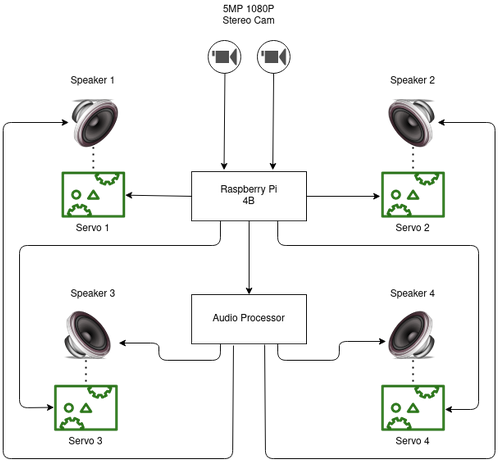
\includegraphics[width=\textwidth]{block_diagram.png}
    \caption{Block diagram}
\end{figure*}

\FloatBarrier

Dynamic audio system can be simplified as five measure blocks, each serving it's
own application in order to provide dynamic surround pocket over the listener's
head,

\section{Depth estimation unit}

Depth estimation unit includes stereo vision assembly of two web cams with similar 
(known or unknown) focal length (In our case 18 cm).

\begin{figure}[h]
    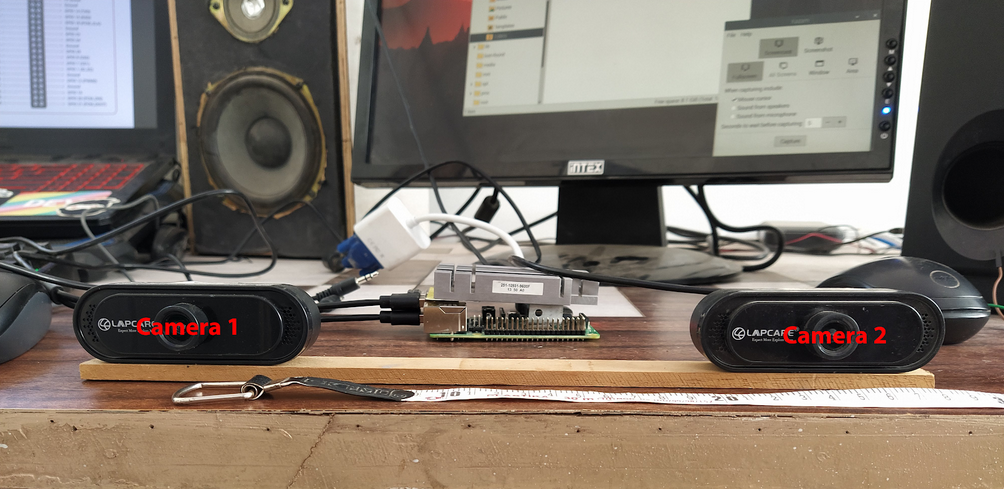
\includegraphics[width=\columnwidth]{assembly.png}
    \caption{Assembly of the depth estimation unit}
\end{figure}

Placed at some known distance \(x \) from each other (24 cm). And implements
computer vision (opencv) and geometrical equations to measure the depth, deviation 
and hieght of a object from a reference point. Where the reference point is the 
center of the stereo vision system.  

\section{Micro-processor}

Micro-processors acts as middleware between DAC and the hardware to control speakers.
In this project we are using raspberry pi 4B (Quad core Cortex-A72 64-bit @ 1.5 GHz clock) 
as our micro-processor. Webcams are connected through USB 2.0 of RPi.

First we find depth, deviation and height of the listener's face from the reference point
using opencv's frontal face harrcascade classifier followed by open source AA symmetry 
algorithm of geometry, where opencv also helps to classify between listener and other objects. 

Above process provides us three real-time variables,

\begin{description}
    \item[1.]Depth of the listener's face from the reference point.
    \item[2.]Deviation of the listener's face from center of the axis.
    \item[3.]Height of the center point of listener's face from the origin (reference point).  
\end{description}

Further using this real-time variables, and some constants (room dimensions and speaker positionings),
using customly designed geometrical algorithm we can calculate, panning and tilting angles, depth of 
the listener from each speaker.

Using panning and tilting angles we can rotate the servos to the required angles to direct the sound field
towards the listener. And using depth we can adjust the sound levels of the speakers by controlling
input voltage of amplifiers digitally.

\section{Mechanical Unit}

As discussed in methodology, as the speakers propagates sound in oval. Hence shape we need to align 
the major axis of the sound field towards the listener.

Mechanical units assembles with, two servo motors for each speaker (channel)
one for panning and second for tilting.

Servos are connected to hardware PWM pins of the RPi and controlled in real time using feedback 
of the angle algorithm.

\section{Audio Processing Unit}

Usually an surround sound system contains two or more speakers in order to generate sound effect
of moving objects from one place to another.

Even if we direct the speakers towards listener's direction, it is encessary to adjust the sound
levels of each speaker according to the depth of the listener from each speaker.

To genrate best surround sound effect, this Audio processor unit assembles with 4 class AB audio 
amplifiers driven by 2 two-channel digital potentiometers for controlling sound levels of each individual speaker to adjust the sound 
pocket over listener's head (ears).

\subsection{Audio amplifier}

Basically, audio amplifier is an circuitrary which is designed to increase magnitude of applied 
signal in order to power a low resistance load (speakers).

Sound signals are applied to non-inverting terminal of an amplifier through an voltage devider
circuitrary (potentiometer). This voltage devider adjusts the voltage levels of the input signal
resulting the change in volume levels at the output. This change is inversly proportional to the
resistance at wiper terminal of the voltage devider.

For this application we are using LM386N-1 as our amplifier.

\subsection{Digital potentiometer}

Digital potentiometers mimics the analog functions of a mechanical potentiometer. Where the resistance
is controlled by micro-controllers or micro-processors.

As we discussed, to adjust the sound output of the audio amplifier we adjust the input voltage given
to the non-inverting terminal of the amplifier. Hence, we supply the audio signal to amplifier through
an digital potentiometer, so we can increase and discrease input voltage and hence the sound 
levels of speaker digitally using a micro-controller or a micro-processor.

For this application we are using SPI compatible MCP42010 Digital POT,

\section{Speakers}

Speakers serves the 4 channeled dynamically adjusted surround sound to the listener. Usually they
are mounted on four corners of the room either at the ear levels of the listener or near the cieling.

\end{document}